% v0.2
\chapter{Modelling bacteriophage genomes}
In this chapter we will present parts of our pipeline intended for data retrieval and preprocessing.
Since we used a considerable amount of third party libraries and tools, we will explain them in detail and we will clarify our reasons for using them.
We will also provide some basic statistics of the data retrieved.

\section{Pipeline overview}
Our pipeline consists of python scripts and publicly available bioinformatics software.
When writing the code, we have taken care of its readability, sustainability and extensibility.

We implemented our pipeline in  workflow management system \emph{Snakemake} \cite{} that was primarily designed for writing reproducible bioinformatics pipelines.
Snakemake is inspired by GNU make, but it uses python-like syntax with elements similar to pseudo code.
Furthermore, it is fully portable, depending only on Python executables and libraries.
Snakefile consists of rules, where each rule is defined by its input files, output files and shell commands.

When the Snakemake is executed, it runs first rule in specified Snakefile.
If the rule is missing input files, it scans through the whole Snakefile and looks for rules that are capable of creating required files.
This process is repeated until there is a rule which can be completed or until there is a rule whose input is not possible to create by any other rule.
In the former case the execution starts running, in the latter case an error message is displayed.
By this approach it is ensured that we do not execute any unnecessary rules nor any rules that have been already completed.
This is an important feature for our program as some rules can take several hours to complete, even on powerful computational cluster.
Another useful characteristic of the Snakemake engine is the ability to produce graphical visualization of particular Snakefile in format of directed acyclic graph.
Simplified graphical representation of our pipeline is in the Figure \ref{fig:dag}.

The pipeline starts with downloading of publicly available data.
After downloading, we merge all records and eliminate duplicated records.
Next, we extract genes of the bacteriophages.
Consequently, phage genomes represented as sets of genes are split into a training and a testing set.
Similarity between the genes from the training set are calculated and based on those, clusters of similar genes are produced.
From these clusters, the binary matrix is created.
This matrix is later used in classification.

\begin{figure}[h]
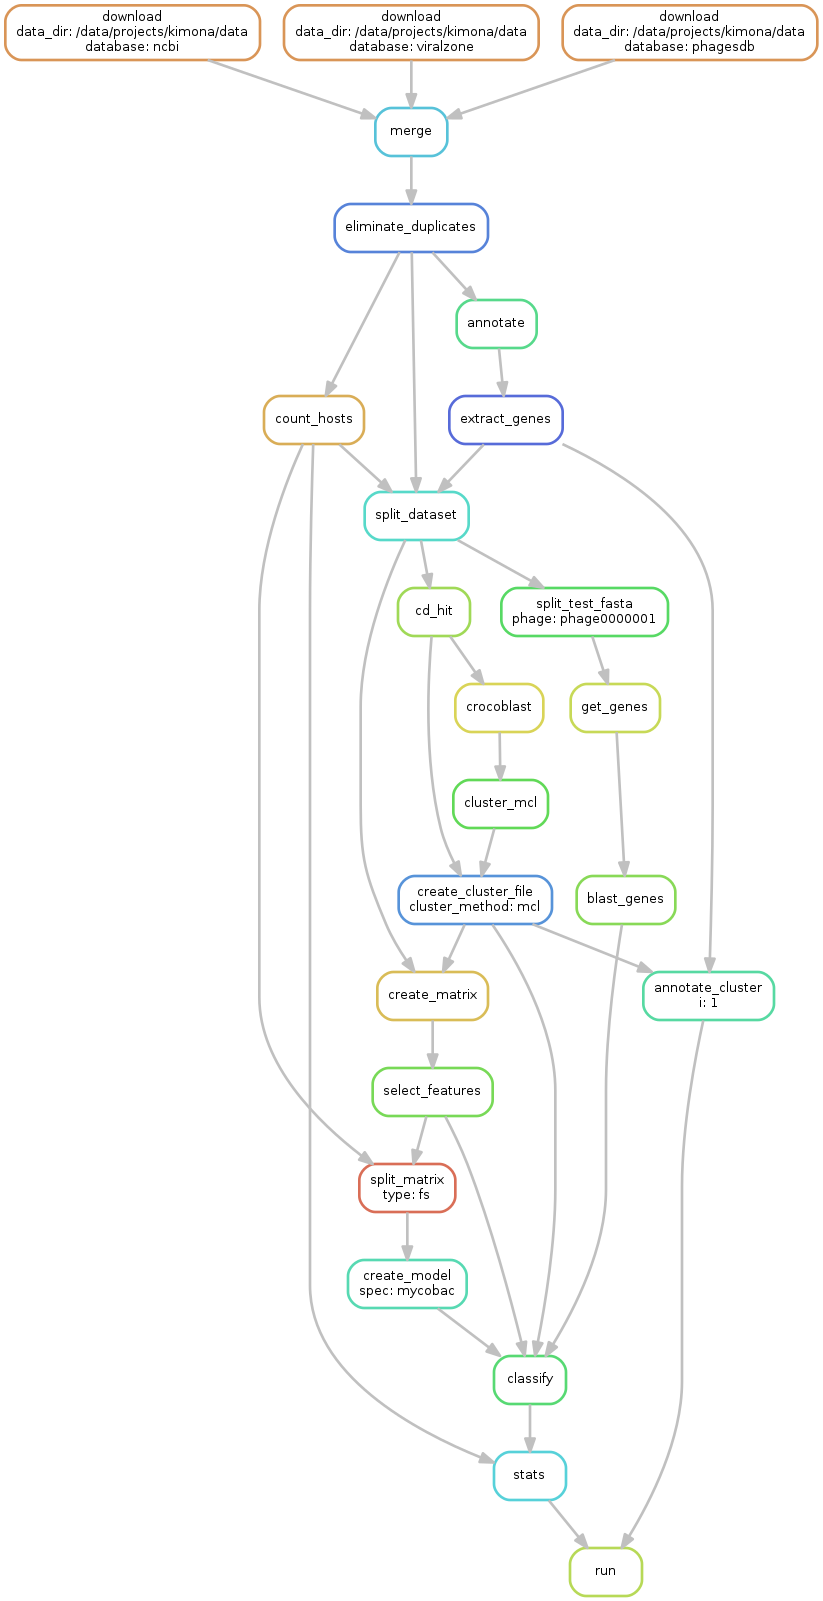
\includegraphics[height=\textheight]{./images/mcl.png}
\centering
\caption{Workflow visualization}
\label{fig:dag}
\end{figure}

\section{Downloading phage genomes}
The first step in our pipeline is downloading of data from three publicly available databases.
Although they cover the majority of currently sequenced and published phages, we made this step easily extensible for adding new sources of information in the future.
New sources can be added by writing a new download script, naming it \verb|{script_dir}\download_from_{db}.py| and appending this name into a variable \verb|DATABASES| in Snakefile.

\subsection{GenBank database}
National Center for Biotechnology Information (NCBI) provides an access to \emph{GenBank}\cite{genbank} database.
This database is a comprehensive source of genomic data with more than 200 million genomic sequences of all life’s domains.
NCBI administers the GenBank database free of charge and give researchers the possibility to access data through various interfaces as web-based retrieval services, FTP and Entrez\cite{entrez}.
Despite of these facts, there are shortcomings of using GenBank.
With recent breakthrough of high-throughput medical technologies the amount of data flowing into GenBank database every day is enormous.
Therefore, it is unreasonable to check all the data.
Sequences are primarily submitted by individuals from all around the globe and are not thouroughly reviewed.
This causes redundancy of sequences and sometimes it even creates contradictions between information in system.

We obtained data using python library Biopython \cite{biopython}, which implements python wrapper NCBI Entrez.
Besides that, we used Biopython to facilitate  processing of standard file formats used in bioinformatics.
When downloading sequences, we also created unique identifiers for each record.
Those were used later in the pipeline.
Reasons behind the decision to use custom identifiers was the ability to remove duplicated sequences and the possibility to find out multiple sources of each sequence in our dataset.
Downloading from GenBank was our largest source of data with 6704 downloaded records.

\subsection{ViralZone database}
ViralZone provides highly reliable data about viruses, including bacteriophages.
Information about the structure of a capsid, a genome, life cycle, replication mechanisms, taxonomy, geographical location and host are included.
This website does not store sequences internally, rather it delivers links to \emph{RefSeq}\cite{refseq} database.
Compared to GenBank, RefSeq database contains fewer sequences, but all of these sequences are curated and manually reviewed.

Our custom script was used to download records from RefSeq database.
Although, large portion of sequences downloaded was identical with GenBank records, some sequences were unique.
Another advantage in performing this action was that it enabled us to pair genomic sequences from RefSeq with more comprehensive information from ViralZone portal.
By performing this process, we obtained 2107 records.

% end of session 2018.04.18
% wc chapter* = 32521 letters

\subsection{PhagesDB}
\emph{PhagesDB} is a database specialized in bacteriophages infecting bacteria from phylum Actinobacteria.
This phylum is of great importance, because of its contribution to the soil system \cite{}.
This phylum also contains the genus Mycobacterium, which includes pathogens causing tuberculosis and leprosy in humans \cite{}.
The database was designed to avoid the time between sequencing and data availability.
Authors declare, at the time of their publication, there was more than 600 records of bacteriophages that were not yet in GenBank.
Furthermore, PhagesDB stores more biologically relevant data , such as discovery details, sequencing details, characterization details, sequence file and a plaque picture.
We downloaded 2491 phage records with our automatized script using the publicly available Application Programming Interface (API).

\subsection{Merging and removing of duplicated records}
Downloaded records were  highly redundant, mainly because many of those records were present in  more databases at once.
To solve this issue, we merged datasets together and removed duplicated records.
For merging we used the standard unix command \verb|cat|.
For removing duplicated sequences, we created a custom Python script.
This script made use of custom identifiers, which were assigned to every sequence that was downloaded.
In case more identical sequences were found, their identifiers were rewritten with the identifier of the first sequence.
This approach preserved the relationships between one particular sequence and all data related to it.
Thus, we were able to track phages, based on their identifiers, to their source databases and also connect them with all data that was already downloaded.
After removing of duplicated sequences our dataset contained 6277 phage records.

\section{Extraction and annotation of genes}
Next step in the pipeline was to identify genes on genomic sequences and annotate them with their biological function.
Although gene annotations of particular genomes are part of genomic records in used databases, we decided to annotate sequences from scratch.
This way we ensured consistency of annotations accross our data .
Another advantage of annotating from scratch is that annotations will always be up-to-date with current human knowledge.

\subsection{Prokka}
We used publicly available pipeline called \emph{Prokka} \cite{prokka} to identify and annotate genes.
First, coordinates of coding DNA sequences (CDS) were found with Prodigal tool\cite{prodigal}.
CDSs are regions of genome that almost always start with AUG codon and end with a stop codon.
These regions can be directly translated into amino acid chains using standard codon table.
After the locations of genes are predicted, Prokka can start to annotate functions of all CDSs.
This is usually done through comparing of a sequence to a database of sequences with an experimentally determined function.
The function of protein with the best match is then assigned to the new CDS.
Prokka, by using this approach searches through multiple databases.
Starting with the most reliable source, which is usually the smallest, it scans all the databases, continuing with the less accurate one.
The databases used with their corresponding order are as follows:
An optional user-defined database, UniProt\cite{uniprot}, RefSeq\cite{refseq}, Pfam\cite{pfam} and TIGRFAM\cite{tigrfam}.
If no match is found across databases, protein is labelled as \verb|hypothetical protein|.

% end of session 2018.04.12
% wc chapter* = 33657 letters

\subsubsection{UniProt}
The UniProt database is acollection of more than 60 million protein sequences and their corresponding detailed information.
Prokka uses just a small fraction of proteins backed up by experimental evidences.
This typically provides information about approximately 50\% of queried proteins.

\subsubsection{RefSeq}
RefSeq, provides information about genomic and protein sequences.
It contains more than 2.5 million protein records.
Multiple sources are integrated in annotation of genes.
Furthermore, all records are curated by the NCBI staff members.

\subsubsection{Pfam}
Pfam is a database consisting of protein families and domain records.
Protein families are groups of protein sharing evolutionary history.
This shared evolutionary history is often expressed by closely related functions and sequence similarity.
Protein domains are parts of a protein sequence responsible for a particular interaction. 
Members of the same protein domain usually share a high sequence similarity.
Protein families and domains are mostly characterized by Profile Hidden Markov Models.
Pfam incorporates more than 6100 of those models.

\subsubsection{TIGRFAM}
TIGRFAM, similarly as Pfam, contains protein families characterized by Profile Hidden Markov Models.
It contains more than 4200 models with comprehensive description of family structure and function.

\vspace{\baselineskip}

All of the aforementioned databases are regularly updated, which guarantees the most up-to-data annotations.
After annotation, resulting genes were selected and saved to files in format suitable for further use in the pipeline.

\section{Datasets used}
At the beginning of this step, our dataset consisted of: phage genomic records, their corresponding genes, information about phage hosts and functional annotation of genes.
As our work used techniques of supervised machine learning, we needed to split the dataset to a \emph{training set} and a \emph{testing set}.
Furthermore, we created set for other records, which we decided not to use due to missing information about host or due to host outside of our group of interest.
We decided to group phages according to the genus of their hosts.
After calculating the number of phages in each group, we selected first eight genera with the highest count of records as groups of our interest.
These were Mycobacterium, Streptococcus, Escherichia, Gordonia, Arthrobacter, Pseudomonas, Lactococcus and Staphylococcus.
Number of phages within each group can be found in the Table (\ref{tab:counts}).
All other genera were excluded from the dataset due to the insufficient number of samples.
Phages without information about their hosts were also excluded.
Subsequently, we divided remaining data into a training set and a testing set at a ratio of 4:1.
The resulting training set included 2787 records of bacteriophages and resulting testing set included 699 records.

\begin{table}
 \centering
        \begin{tabular}{ l  r  l  r }
         \hline
         genera & count & genera & count \\
         \hline
         Mycobacterium & 1619 & Streptococcus & 354 \\
         Escherichia & 323 & Gordonia & 293 \\
         Arthrobacter & 240 & Pseudomonas & 236 \\
         Lactococcus & 219 & Staphylococcus & 184 \\
         \hline
        \end{tabular}
        \caption{Counts of records within genera}
        \label{tab:counts}
\end{table}

%--------deeply described parts-------------------------------------------------
\section{Alignment in the pipeline}
In our pipeline, we used alignment to find similarity scores between genes in the training set.
We needed these scores later in the pipeline at clustering step.
Software CrocoBLAST \cite{} was used for this purpose.
CrocoBLAST is a wrapper around BLAST algorithm which makes better use of parallelization than standard BLAST maintained by NCBI.
With this software we were able to reduce the time needed for the alignment step from around four days to one day.
Resulting file was in tab separated format, where first column was gene identifier of query sequence, second column was gene identifier of the target sequence and third column was e-value of alignment.

\section{Clustering in our pipeline}
\subsection{MCL}
Firstly, we used Markov Cluster Algorithm implemented in package MCL \cite{mcl}.
This software is popular in the bioinformatics community for its capabilities to work with big data.
As input data we used E-values from CrocoBLAST results.
These E-values were automatically transformed into a similarity score to enable creation of the adjacency matrix.
We used the value 1.2 as the inflation parameter.
This was the smallest value recommended by the developers.
The reason for using the smallest possible inflation value was that we wanted to create clusters that are as large as possible
This approach also reduced the number of different clusters.
In our work, we needed as few clusters as possible, mainly due to the number of phage records in our dataset.
If we had too many clusters, we would have too many features for classifier and we would risk overfitting of our final models to the training dataset.
We created 15017 gene clusters.

\subsection{MCL with global alignment}
To get more accurate clustering, we tried different approach, where we determined similarity score from the global alignment.
All the matches from CrocoBLAST search were aligned with the needleman-wunsch algorithm \cite{needleman-wunsch} and the resulting score of alignment was used instead of the E-value.
Implementation of the Markov Cluster Algorithm was executed with an inflation parameter value of 1.2, without any transformation of the similarity score.
By this approach we created 9176 final clusters.

\subsection{Spectral clustering}
In this work, we also experimented with a different clustering algorithm, Spectral clustering.
SCPS implementation\cite{scps} was tested in the pipeline.
Although authors of this software declare quality of clusters quantified by a measure that combines sensitivity and specificity to be better by 28\% in comparison to MCL algorithm, our memory was not sufficient for the program to run with all the input data.
%--------end of deeply described parts------------------------------------------

\section{Annotation of gene clusters}
Clusters of genes were annotated to determine their function.
We expected proteins with similar biological function to be included in same cluster.
For functional annotation of particular proteins we used software \emph{InterProScan} \cite{interpro}.
This tool scans given protein sequences against the protein signatures in databases PROSITE \cite{prosite}, PRINTS \cite{prints}, Pfam \cite{pfam}, ProDom \cite{prodom} and SMART \cite{smart}.
After acquiring of annotations for all proteins in a particular cluster, we calculated number of occurrences of each distinct biological function.
These statistics represent our annotation of a certain cluster.
Our expectation of clusters containing proteins with similar function was met in most cases, although the information about particular proteins were sparse with a lot of proteins without any information.
Therefore, we assumed that reasonable clustering was achieved.

\section{Reducing phage genomes}
One of the most crucial part of our analysis was \emph{binary matrix} created in this step.
Rows in this matrix represented particular phage records and columns represented particular protein clusters.
The entry $a_{i,j}$ in matrix was filled with $1$ if phage $i$ contained gene from cluster $j$ and $0$ otherwise.
Custom python script and files produced in previous steps were used for this task.
Resulting matrix contained 2787 rows and 15017 columns and served as a main input file for the machine learning algorithms.